\documentclass{llncs} % , times

\usepackage{amssymb, amsmath, graphicx, ltxtable, longtable, tabularx, url, ragged2e, xspace, verbatim, fancybox,tikz}
\usepackage{scalefnt}
\usepackage{relsize}
\usepackage{paralist}
\usepackage{listings}

\usepackage{tikz} 


\newcommand{\ggr}[1]{\textcolor{magenta}{comment Gerd: \textit{#1}}}

\lstdefinestyle{code}{language=java,
        numbers=left,
        xleftmargin=1em,
        numberstyle=\tiny,
        showstringspaces=false,
        frame=single,
        basicstyle=\ttfamily\footnotesize,
        escapeinside={(*@}{@*)}
        }

\lstdefinestyle{rdfexample}{
	numbers=left,
	numberstyle=\tiny,
	%numbersep=0.1pt,
	xleftmargin=2em,
	showstringspaces=false,
	frame=leftline,
	basicstyle=\ttfamily\small,
        escapeinside={(*@}{@*)}
	}


\newcommand{\fs}{\textsf{F\#}\xspace}

\newcommand{\rr}[1]{\textbf{RR #1}}

%\newcommand{\nr}[1]{
%\begin{tikzpicture}[auto,node distance=1cm,thin] 
  %\tikzstyle{every node}=[shape=circle,draw=none, 
    %text=black] 
  %\node (1) {\texttt{NR #1}}; 
%\end{tikzpicture} }
%
%\newcommand{\tr}[1]{
%\begin{tikzpicture}[auto,node distance=1cm,thin] 
  %\tikzstyle{every node}=[shape=circle,draw=none, 
    %text=white,shading=ball] 
  %\node (1) {\texttt{TR #1}}; 
%\end{tikzpicture} }

\newcommand{\tr}[1]{\textbf{TR #1}}

%\newcommand{\rdfs}[3]{\textbf{#1}: $\frac{#2}{#3}$}
\newcommand{\rdfs}[3]{\textbf{#1}: $\frac{\texttt{#2}}{\texttt{#3}}$}

\pagenumbering{arabic}

\begin{document}
\title{Improving Programmability of Linked Data Sources}
 





\author{Gerd Groener\inst{1}, Kenji~Takeda\inst{2}, Don Syme\inst{2}, Ross McKinlay\inst{2}}
%\\ \textsf{groener@uni-koblenz.de}}

\institute{$^1$Institute for Web Science and Technologies, University of Koblenz-Landau, Germany \\
$^2$Microsoft Research Cambridge, UK}

%\institute{Institute for Web Science and Technologies\\
%University of Koblenz-Landau, Germany}

\maketitle

\begin{abstract}

\end{abstract}


%Information in RDF data sources is given by a set of explicit statements.
%Additionally,  RDF inference consists of a set of rules to derive
%implicit information from RDF data. This inference relies on
%the data structure. When processing data in
%programs and workflows, further information like type statements
%can be derived based on the flow of the data. 
%In this paper, we present an integration of RDF inference in
%a data processing environment. 

%%%%%%%%%%%%%%%%%%%%%%%%%%%%%%%%%%%%%%%%%%
\section{TODO: Proposals for title}

Some ideas for the title:
\begin{itemize}
	 \item Towards a Data-oriented Type System in Programming Environments

   \item A type Bridging technique for RDF data sources
	
	  \item Adapter Layer for Web data integration

   \item Connected Programming
\end{itemize}


%%%%%%%%%%%%%%%%%%%%%%%%%%%%%%%%%%%%%%%%%%%%%%%%%%%%%%%%%%%%%%%%%%%%%%%%%%%%%%%%%%
\section{Introduction}
\label{sec:intro}
%%%%%%%%%%%%%%%%%%%%%%%%%%%%%%%%%%%%%%%%%%%%%%%%%%%%%%%%%%%%%%%%%%%%%%%%%%%%%%%%%%%%%%

% we just want to improve the programmability in web applications for linked data

% problem
Publishing linked (open) data on the Web has become a success story during the last years.
RDF as the underlying representation formalism allows for flexible modeling of data such that
users are able to easily share, distribute and interconnect their own data all over the world.
Publishing and representing data on the Web is one side of the coin, but writing programs
and applications that access and smoothly integrate RDF data  is another, rather challenging issue.

One key problem is the fundamental gap how data is processed in both areas.
RDF representation benefits from the flexible data model,
while software engineering environments and programming languages rely on powerful typing mechanisms
that guide programmers in their development by intelligent IDE support
and avoid run-time exceptions that might be caused by incompatible types.


% interesting
The integration of large external data into programs and programming environments
has already been investigated by dynamically typed programming languages.
However, as it is in the nature of these languages, without type support when writing program code.
Some initially approaches use adapter mechanism to integrate large data sources into statically
typed programs. They rely on a rigit and well-known schema of the data source.
Given such schema information, these approaches have led to good principles and toolins to
allow for a smooth integration of data.

Looking into linked data, the question arises whether
a smooth integration is even possible for RDF data sources.
In particular, we are faced with the following problems.
First, schema information might be partially unknown and even incomplete when data are accesses.
Instead, the structure among individuals, which is given in terms of properties between individuals,
might be used for a data access with respect to a certain structure.
Second, while the schema is rather fix, the underlying data tend to change rather often.
Thus, programs at run time might incorporate such aspects.
Third, the sheer size of data sources (like DBpedia)  might lead to a large number of types
and accordingly to high type generation effort, while the program and system execution
only need a part of the generated types.
Thus, in an extreme case, this might even make the use of statically typed languages impossible.


%At a first glance, an alignment between schema information in RDF (RDFS) and types in programming languages
%is a rather straightforward means to allow for typing of data from RDF sources in program execution.
%This is even a rather fix ``bridge'' since the schema in RDF sources tend to change rarely,
%which is necessary for a stable type system.
%However, at program run-time, there is no straightforward way how to incorporate implicit,
%incomplete and steadily changing data from RDF sources within the execution of (statically) typed programs.
%
%%hard
%Integrating Web data sources into types programming environments is a rather challenging problem.
%First, data sources on the Web might be huge and are often connected to other sources and thus.
%
%(i) data change at run time
%(ii) representations might be incomplete
%(iii) data-oriented representation vs. class centric modeling
%
%
%% related work
%Existing approaches: Type Provider
% Contribution

In this paper, we present an integration and type bridge from RDF data sources to
statically typed programming languages. We adopt the principles of \emph{type provider}
to define an adapter in terms af a library (i.e., a dll-file) for statically typed programming languages. This adapter can
be loaded in a program to access an arbitrary RDF data source that offers a SPARQL endpoint.


%%%%%%%%%%%%%%%%%%%%%%%%%%%%%%%%%%%%%%%%%%%%%%%%%%%%%%%%%%%%%%%%
%\section{Use Case and Application Context}
%\section{Context and Problem Description}
\section{What does programming Linked Data mean?}
\label{sec:context}
%%%%%%%%%%%%%%%%%%%%%%%%%%%%%%%%%%%%%%%%%%%%%%%%%%%%%%%%%%%%%%%%%%%%%%%%%%%%%%%%%%%%%%%%%%%%%%%%%%%%


The RDF data model is basically a graph, which is constitued of a set of subject-predicate-object triples.
This graph covers both the schema in terms of classes and the data in terms of individuals
The usage of certain predicates like \textsf{rdf:type}, \textsf{rdfs:domain} and \textsf{rdfs:range}
and classes like \textsf{rdf:Class} indicate that certain entities in the graph are classes.
Thus, this is the only evidance for a schema.


\subsection{Examplified Problem Description}

When writing programs and Web applications, programmers use programming languages and environments like IDEs
the write their code. 
Programming languages typically rely on some kind of schema or types
where types (or classes) serve as containers to manage data.
The organization of types in a so-called type system is an essential benefit of \emph{statically typed} languages where a powerful type system support programmers during the program design and 
ensure type correctness in program execution. In particular, statically typed programming languages provide the following benefits:


\begin{enumerate}
	\item \textbf{Design Time Assistance:} The programming environment provides support programmers when writing code by
	 context-sensitive auto-completion, interactive type checking (so called red squigglies) and quick information display like mouse-hover
	and detailed documentation (e.g., by pressing F1 button). All these interactive features help programmers in writing their code
	and give early feedback (at design time) about program correctness. 
	\item \textbf{Run Time Assistance:} When a statically program is compiled, type definitions and their usage in programs
	        are checked. Thus, at run time, we can rely on a proper type system that offers features like type casts,
					 type checking and type inference. Run time errors and exceptions during program execution based on
					 incorrect type usage and type mismatch are already detected during design and compilation, and thus, might not
					cause errors at run time. Types can be even used to optimize type interpretations.
					\ggr{I can't remember what the last sentence about optimize / drive interpretations mean.}
					
\end{enumerate}

While these benefits of statically typed programming languages are obvious,
the key question is how can such features be achieved when we access and integration RDF data sources,
i.e., types in our type system refer to RDF classes and collections of individuals.
This means, that types are used in the usual programming manner, for instance RDF individuals
have all properties that are defined by the RDF classes. This is illustrated in the following example.
In each step, we see the corresponding requirement that has to be addressed by a type bridge.
We can distinguish between \emph{retrieval requirements (RR)} and \emph{typing requirements (TR)}.

Assume a developer is programming an application for a mobile phone to provide additional
data for movies like information about actors or genre. These additional data
are retrieved from RDF data sources like DBpedia\footnote{DBpedia: \url{http://dbpedia.org}} via a SPARQL endpoint,
e.g., as provided by DBpedia\footnote{DBpedia SPARQL Endpoint: \url{http://dbpedia.org/sparql}}.
These data should be included in the application on demand, i.e., only if needed
and they should be managed in the application in a typed fashion,
as described above.

\vspace{0.8em}
\noindent
\textbf{Step 1: Find a Class.}
First of all, the programmer decides to use DBpedia as a data source since it is well connected to other
data sources. As a first step, the programmer has to look for a dedicated class for ``Actor'' in the data source.
For this purpose, the data source must be explored, e.g., by showing all RDF classes in a list
such that the developer can select the class of interest.

\rr{1}: Thus, we need means to explore a data source in terms of retrieving classes in RDF data sources.

\vspace{0.8em}
\noindent
\textbf{Step 2: Define a Class / Type for  an RDF Class.}
Once, a class for an ``Actor'' is found, e.g., \texttt{http://dbpedia.org/ontology/Actor}, the programmer has
to define this class in the program.

\begin{lstlisting}[style=code, caption={Type Definition for RDF Class ``Movie''}, label={lst:movietype}]

// Type definition for "Actor" 
type Actor = {
  id : URI
  rdfs:label : String 
}
\end{lstlisting}

\tr{1}: The problem we have to solve here is to map the RDF class description into a type definition in the program code.

\vspace{0.8em}
\noindent
\textbf{Step 3: Define Related Types.}
Looking into the RDF class, we see that ``Actor'' is a subclass of ``Artist'' (\texttt{http://dbpedia.org/dbpedia-owl:Artist}).
Hence, if we want to reflect this characteristic, we need to define a type for class ``Artist'' too.

\begin{lstlisting}[style=code, caption={Type Definition for RDF Classes ``Actor'' and ``Artist''}, label={lst:worktype}]

// The "Artist" Type
type Artist = {
  id : URI
  rdfs:label : String
}

// Again the "Actor" Type as Subclass of "Artist"
type Actor = {
  inherit Work
  id : URI
  rdfs:label : String
}
\end{lstlisting}


Obviously, besides the ``Artist'' class, other class might be created as Movie is related to them. This procedure might even continue since
these other classes like ``Artist'' can depend on other classes.

Given the sheer size of linked data sources (or even the linked data cloud), the key \emph{problem} is which classes need to be 
integrated in a program, i.e., for which RDF classes is a type definition necessary. Building types for all classes of a
data source is definitely not scalable, ane even not needed since a particular application 
might only a part of the classes.

\tr{2}: Thus, the question is whether it is possible to build types only \emph{on demand}.

\vspace{0.8em}
\noindent
\textbf{Step 4: Define individuals of classes.}
In our application, we want to mange concrete movies, which can be derived from the data sources,
as individuals of this class. Using a SPARQL query we can retrieve all individuals of class ``Actor''.
For instance, we get the individual \texttt{http://dbpedia.org/page/Bruce\_Lee} for the actor ``Burce Lee''.
Accordingly, we can build an instance of movie.

\begin{lstlisting}[style=code, caption={Individual of  ``Actor'' }, label={lst:skyfall}]
let bl = Actor(`http://dbpedia.org/page/Bruce_Lee')
\end{lstlisting}

\tr{3} Types are used to instantiate individuals. 

\vspace{0.8em}
\noindent
\textbf{Step 5: Incorporate Properties of Individuals.}
It is in the nature of the flexible RDF model that properties can be defined for individuals 
without explicit definition of these properties for classes. For instance, the individual
``Burce Lee'' has properties that are not specified for stated as properties for the RDF class ``Actor''.

\tr{4} and \rr{2}: Incorporating properties of individuals at the type level. From a programming language perspective,
this is a rather callenging issue since a type usually specifies properties, which can be even optional,
but in our case, the previously sketched type specification does not even know about additional properties.


%requires means for bridging between the data representation on the Web and 
%Assume data from Wikipedia should be incorporated in an application, e.g., a touristic company makes
%to use published and up-to-date data about cities, landscapes and prominent people that are associated with citites.
%To do this, the company decides to retrieve data from DBpedia and and completely include / integrate these
%data in their programs.
%When writing programs and Web applications that access these data and especially integrate them such that they
%In general, connecting and integrating information spaces in programming languages is an essential part on informaiton-rich programming.
%One of the most prominent source is DBpedia, where
%parts of Wikipedia data are represeted as RDF,  and access to these data is offered via SPARQL endpoints. 
%The linked data cloud is mainly accessibly by SPARQL requests, retrieving
%classes (schema information) and data.
%However, the integration of data into a statically typed programming language is more than querying a data source.



% figure system architecture


%%%%%%%%%%%%%%%%%%%%%%%%%%%%%%%%%%%%%%%%%%%%%%%%%%%%%%%%%%%%%%%%%%%%%%%%%%%%%
\subsection{Contribution}
%%%%%%%%%%%%%%%%%%%%%%%%%%%%%%%%%%%%%%%%%%%%%%%%%%%%%%%%%%%%%%%%%%%%%%%%

We distinguish between contributions 
that are related to (i) the programming environment, (ii)~ the mapping from
schema and data requests to SPARQL queries and (iii)~the Semantic Web and linked data
oriented investigations.

%\subsection*{Programming Language and Environment}

We present a type bridge or type adapter in order to create types for RDF classes that
are retrieved from linked data sources. 
In essence, the type bridge acts as a type provider in \fs that support the integration of information sources
into \fs~\cite{Syme2012fsharp}. Type provider are means for data progamming
in statically typed programming languages.
The general principle of type providers is 
to retrieve a well structured schema from (Web) data sources in order to build
the corresponding types at run-time.

In our case, we can not rely on a well structured schema, thus we have to
incorporate RDF modeling characterisits in order to integrate data into
a static type system. The closed related type bridge is the Freebase  
type provider that allows for the navigation within the graph-structure of
Freebase~\footnote{The Freebase Wiki about the Schema: \url{http://wiki.freebase.com/wiki/Schema}}.

The RDF type bridge includes the following aspects.


\paragraph*{\bf Type Integration and Type Inference.}
When deriving RDF data from external data sources, the key problem is how to integrate
such types into the host programming schema. \\
\textbf{Contribution:} Types are built based on the schema information that is obtained
from the RDF data source. The schema is derived by the 
usage of certain predicates like \texttt{rdf:type}, \texttt{rdfs:domain} and \texttt{rdfs:range}
and classes like \texttt{rdf:Class}.

\paragraph{\bf Scalable Type Definition on Demand.}
As data sources on the Web tend to be huge, it is not a promising idea to
build the types for all classes of a data source.
Obviously, types are only needed if particular applications need to access them.
\textbf{Contribution:} On demand typing based on the current element. \\


\paragraph*{\bf Incorporate Data Changes.}
It is obvious that RDF data change rather frequently, while the
schema remains stable. Thus, it is meaningful to build types wrt.\ schema (at design time)
and populate these types at run time.\\
\textbf{Contribution:} Types are built wrt.\ the schema (class definitions in RDF).
Classes are populated by individuals at run time.
This implicitly also takes changes of the data (individuals) into account. \\


%\subsection*{Semantic Web and Linked Data}


\paragraph*{\bf Derive fine-grained Schema from RDF Data.}
Hierarchies of classes and also properties in RDF data can be quite extensive.
Besides this, domain and range restrictions of properties that entities can be classes
in case this is not explicitly stated. \\
\textbf{Contribution:} We incorporate RDF entailment regime, which is supported by SPARQL~1.1
in order to derive a fine-grained type system / schema.
While our type bridge is built to access and integrate RDF data into programs,
we also use Semantic Web technologies and built the data access upon
these existing means. In particular, we apply SPARQL queries, the SPARQL entailment regime, which
includes RDF(S) entailment, and we actually rely on best practices for publishing linked data.


\paragraph*{\bf Retrieval on Class vs. Instance level.}
In RDF data sources, property specifications at the class level are often rare,
for instance in DBpedia classes have only three or four properties and these are actually
quite generic one, derived from super-classes. Instead, the most interesting way for navigating
is at the instance level. But, how can we cover properties if their corresponding class
in the programming language does not have this property. We can even not assume this property
for the class since the individuals do not necessarily share their properties. \\
\textbf{Contribution:}  We offer a two-layered navigation in RDF sources.

%\paragraph*{\bf Retrieval on Class vs. Instance level.}
%In RDF data sources, property specifications at the class level are often rare,
%for instance in DBpedia classes have only three or four properties and these are actually
%quite generic one, derived from super-classes. Instead, the most interesting way for navigating
%is at the instance level. But, how can we cover properties if their corresponding class
%in the programming language does not have this property. We can even not assume this property
%for the class since the individuals do not necessarily share their properties. \\
%\textbf{Contribution:}  We offer a two-layered navigation in RDF sources.



%\paragraph*{\bf Property-based Classes.}
%RDF data have type statements that assign data (individuals) to classes.
%However, it has been shown that besides the type statements
%properties of individuals are an essential means to group individual to a kind of
%classes instead of only relying on explicitly specified types. \\
%\textbf{Contribution:} We allow the specification of types as a set of properties. \\
%
%
%\paragraph*{\bf Set-based Classes.}
%Following the OWL-based set semantics, classes in the RDF sense can be considered as
%unions or intersections of RDF classes. \\
%\textbf{Contribution:} We allow the specification of types as a unions and intersection of existing types. \\
%
%
%\subsection{Semantic Web and Linked Data}
%
%\ggr{not sure, whether the mapping to SPARQL is worth to mention.}



%%%%%%%%%%%%%%%%%%%%%%%%%%%%%%%%%%%%%%%%%%%%%%%%%%%%%%%%%%%%%%%%%%%%%%%%%%%%%%%%%%%%%%%%%%%%%%%%%%%%%%%%
\section{Foundations}

%%%%%%%%%%%%%%%%%%%%%%%%%%%%%%%%%%%%%%%%%%%%%%%%%%%%%%%%%%%%%%%%%%%%%%%%%%%%%%%%%%%%%%%%%%%%%%%%%%%

An RDF\footnote{RDF Primer: \url{http://www.w3.org/TR/rdf-primer}} data source consists of at least one RDF graph, which is a set of RDF triples $(s, p, o)$
that consists of subject (s), predicate or (p)  and object (cf.~Def.~\ref{def:rdf}).

\begin{definition}[RDF Graph]
\label{def:rdf}
Let $U$ be a set of URIs, $L$  a set of literals and $B$ a set of blank nodes,
with $U \cap L \cap B = \emptyset$.

An RDF graph is defined as:
$\mathrm{G}$ $=$ $\{ (s ,\ p , \ o) \in (U\cup B)\times U \times (U\cup L \cup B) \} $. 
\end{definition}


SPARQL\footnote{SPARQL 1.1 Query Language: \url{http://www.w3.org/TR/sparql11-query}} 
is a query language for RDF graphs with  \textsf{select}, \textsf{from} and \textsf{where} clauses.
Like an RDF graph, the graph pattern of the \textsf{where} clause consists of RDF triples, in which
variables are allowed as subjects, predicates and objects of triples.
The result of a query is a binding of the variables in the \textsf{select} clause,
while the binding is determined by matching of triples from the \textsf{where} clause
to triples in the RDF graph $G$.

In SPARQL 1.1, which we are referring to in this paper, the graph matching principle between triples in the query and the data source
is extended by entailment relations, as defined by the SPARQL entailment regimes\footnote{SPARQL 1.1 Entailment Regimes:
\url{http://www.w3.org/TR/sparql11-entailment}}. Among others, the entailment regimes contain RDF and RDFS entailment rules
Thus, triple matching is extended to triples that can be derived from an RDF graph $G$. Formally, we denote
this extended set of triples, which can be derived by RDF(S) entailment, as Materialized Graph (cf.~Def.~\ref{def:mat}.A).
(The symbol $\models_{\mathcal{T}}$ denotes RDF(S) entailment.)

We use a distinction between classes (schema) and data in the RDF graph.
We refer an entitiy $C$ (subject or predicate in a triple) as a class (or RDF class).
This is described in Def.~\ref{def:mat}.B.
 

\begin{definition}[Materialized RDF Graph and RDF Classes]
\label{def:mat}
Let $\mathrm{G}$ be an RDF graph.
\begin{itemize}
	\item[A.]  A materialzed graph $\hat{G}$ is defined as follows:

$\hat{G}$ $=$ $\{ (s ,\ p , \ o) \in (U\cup B)\times U \times (U\cup L \cup B) \ | \ G \models_{\mathcal{T}} (s, \ p, \ o) \}  $. 

\item[B.] $C$ is referred to as a class (or RDF class) if one of the following conditions hold:
(i) there is a type statement  (s rdf:type C) $\in \hat{G}$,
 (ii) there is a domain restriction (s rdfs:domain C) $\in \hat{G}$ or 
(iii) there is a range restriction (s rdfs:range C) $\in \hat{C}$ and C is not a datatype.
\end{itemize}
\end{definition}



%These rules derive implicit relations between classes, individuals and classes for individuals (\textsf{instanceOf} relation) based
%on explicit stated relations and domain and range restrictions of properties.

Foundations: \fs and Type Provider

\begin{definition}[Type System]
\label{def:type}
A type system is a tuple $(\Gamma, \mathcal{T})$
Let $\Gamma$ be a domain,  $\mathcal{T}$ a set of type expressions (or types for short).
$\top \in \mathcal{T}$ is the most general type expression that is a super-type of all other types.

For each element in the domain $e \in \Gamma$ there is a type $\tau \in \mathcal{T}$ such
that $e$ is an individual of type $\tau$: $e: \tau$
\end{definition}


\begin{definition}[Class-Type Mapping]
\label{def:map}
An RDF graph $G$ is mapped to a type system $(\Gamma, \mathcal{T})$ by a class-type mapping $m$.
Each (named) RDF class $C$ is mapped to a type $\tau \in \mathcal{T}$. Each
property is mapped to a type tuple $(\tau_1, \tau_2) \in \mathcal{T} \times \mathcal{T}$.\footnote{Note: If
the domain or range class of a property is unknown, the corresponding types are $\top$.}
\end{definition}


%%%%%%%%%%%%%%%%%%%%%%%%%%%%%%%%%%%%%%%%%%%%%%%%%%%%%%%%%%%%%%%%%%%%%%%%%%%%%%
\section{A Type Bridge for RDF}  
\label{sec:design}
%%%%%%%%%%%%%%%%%%%%%%%%%%%%%%%%%%%%%%%%%%%%%%%%%%%%%%%%%%%%%%%%%%%%%%%%%%%%%%

\ggr{not sure we use `bridge', `adapter' or `type provider'?}

\ggr{we have to make the distinction clear: (i) the work we did (meta-level) and (ii) how the TP is used as a library (run time)}

Our goal ist to build an integration bridge for arbitrary RDF data sources with a SPARQL endpoint
in order to access and integrated RDF data into a statically typed program on demand.
When using these bridge, it should not be part of the actual developed application,
instead it is just used as a library. In the following, we will see some technical details how
the bridge is developed.

\subsection{Features of the Type Bridge}
  
According to Sect.~\ref{sec:context}, we aim at achieving two groups of requirements:
retrieval requirements (RR) and typing requirements (TR). Navigation is needed since the an RDF graph does not explicitly 
distinguish between schema and data, as for instance in relational databases. Thus, the navigation is
used to find those elements in the graph that should be integrated as types and their corresonding data (individuals) in a program.
Aspects of the integration into the programming type system are reflected by the typing requirments (TR).

In order to meet the requirements, the type bridge has to provide the following functionality.
First, the exploration of an RDF graph must be supported. Thus, we need some kind of data handler
to be able to hook into the RDF source. Second, we have to use the data handler to explore the data source by
following the properties from one entity to the next one. This must be provoded for RDF classes and individuals.
Properties also include type statements, and therefore,
we can also follow relations between classes and individuals.
Third, the retrieval of the currently explored entity and its properties must be supported.
Fourth, The definition of a static type must be soported. This means that also all properties of
the type must be defined.
The type bridge, its features and its context of use is illustrated in Fig.~\ref{fig:context}.
The design and implementation of the type bridge is described in the next part of this section.

\begin{figure}
	\centering
		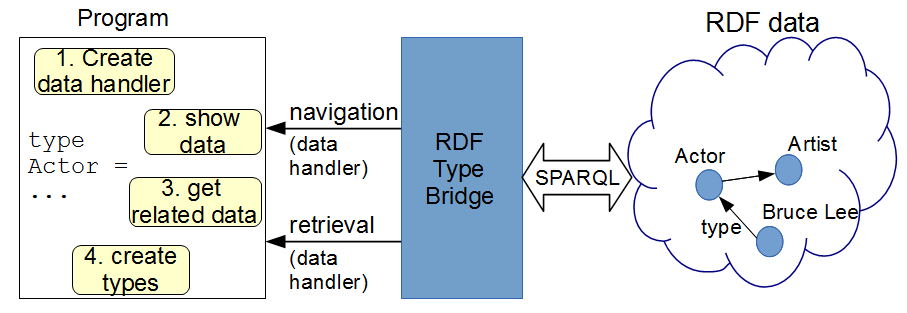
\includegraphics[width=0.98\linewidth]{./figs/context.png}
	\caption{Functionality and Context of the Type Bridge}
	\label{fig:context}
\end{figure}



\subsection{Type Definitions}

Our type bridge is a compile time component. It has static parameters like
the address (URI) of the SPARQL endpoint.
The type bridge consists of two components: (i)~the data source \emph{connector} and (ii)~the
\emph{type generation description}. The latter one is a kind of compile-time meta-programming construct.
In the following, we consider both components in detail.

The \emph{connector} establishes a connection to the SPARQL endpoint. It serves as a mediator
between the type generation descrition and the external data source.
The connector gets as an argument the URI of the SPARQL enpoint
in order to establish a connection to the SPARQL endpoint.

All data are obatined from the data source by SPARQL queries.
Thus, the connector consists of functions that are used by the type generation description
to navigate in the data source and to retrieve data from the source.
Internally, these functions encode SPARQL queries in order to implement both tasks the navigation and the retrieval.

Functions of the connector are used to retrieve (i)~all classes of the source,
(ii)~individuals of a certain class, (iii)~properties of a class (i.e., the objects of
triples in which the class is the subject and the property the predicate),
(iv)~properties of an individual and (v)~the classes of an individual.
The notion of a class in the RDF data referes to the specification of Def.~\ref{def:mat}.
%
%
%After a successful connection to the SPARQL endpoint, we get the following 
%artefacts for data access and connection:
%
%\begin{enumerate}
	%\item The \emph{signature} of the data source, which is given by classes and properties in 
	  %the data source, is retrieved.  \ggr{not really retrieved --- can be retrieved}
	%\item The \emph{type creating} on  demand.
%\end{enumerate}	



The key part of the type bridge is the \emph{type generation description} that
defines how types with their parameters, properties and methods are built when the bridge is used.
In essence, the type bridge is model that specifies the type import into a programming language.
In the following, we discuss the key rules for the type import of an RDF type bridge.

The first part is the definition of the type itself, which represents an RDF class from the data source.
The rule spcifies how the programming language has to define a type for an RDF class.
The type definition requires at least the name of the type and its erasure, i.e., the type this type can be erased to.

Let C be the class, which is retrieved by a SPARQL query. The type generation description in \fs
is as follows:

\begin{lstlisting}[style=code, caption={\textbf{Type Rule:} Type Generation Description for RDF Class C}, label={lst:providedClass}]
t = ProvidedTypeDefinition(cname, baseType=Some typeof<obj>)
\end{lstlisting}

In Listing~\ref{lst:providedClass}, \texttt{cname} denotes the name of class $C$, e.g., this can be the string of the URI of $C$.
The \texttt{baseType} gives the erased type, a``super-type'' from which the generated type $t$ inherits.
For instance, an RDF class can just be erased to an \fs object type. If a type should have other features
like being iterable, the type can be erased to sequence or list and thus, this type can serve as a collection
element and iteration features on its elements will part of the type characteristics.

As an example, assume we specify a type generation description for RDF classes.
This description, which is a compile-time meta-programming constuct, is
used to build RDF classes, e.g., the ``Actor'' class in our example.


Types can have properties. Accordingly, if a type will be created, the corresponding properties
have to be created too. These properties are obtained from the RDF data source and should
be directly reflected in the source code that will specify the corresponding type.
Accordingly, the type generation description describes how to obtain properties and to
generate the properties of these types.

\begin{lstlisting}[style=code, caption={\texttt{Property Rule:} Add Property for Class C}, label={lst:providedProp}]
 let p = ProvidedProperty(pname, typeof<string>, 
    GetterCode = (fun args -> 
		     <@@(%%(args.[0]):obj) :?> string  @@>))
  // add this property (delayed)
 t.AddMemberDelayed(p)
 \end{lstlisting}

In Listing~\ref{lst:providedProp}, \texttt{pname} denotes the name of the property (e.g., the URI), \texttt{typeof} gives the
super-type (string in this case) and \texttt{GetterCode} is a so-called quotation that specifies the result of a property selection at run time.
In this simple case, the string representation of the property itself is the meaning of the property.

In the second line, the peroperty is ``added'' to the type. Note, this this depends on the concrete generated type 
when the bridge is used in a concrete program. For instance, if a type for RDF class ``Actor'' is created (according to the rule in Listing~\ref{lst:providedClass}),
the properties (predicates in the RDF graph) of ``Actor'' are generated and added (according to the property rule in Listing~\ref{lstProvidedProp}).

In the next rule, we treat individuals. They can be added to their corresponding classes.
The according type description specification is shown in Listing~\ref{lst:providedIndColl}.
For this, a new type would be created with the name of the class (denoted by \texttt{cname}) and the
suffix ``Individuals''. This type is added to t. In this collection, all individuals are contained.

\begin{lstlisting}[style=code, caption={\texttt{Individual Rule:} Add Individuals (set / collection) to Class C}, label={lst:providedIndColl}]
let individuals = 
   ProvidedTypeDefinition(cname+"Individuals", Some typeof<obj>)
\\ add these individuals
individuals.AddMembersDelayed()
\\  add indiviual collection to type 
t.AddMemberDelayed(indiviuals)
 \end{lstlisting}

Like classes, individuals can have properties too. This means we are looking for properties $p$ where
the individual $i$ is the subject of a triple: $(i, p, x)$. The specification is shown in Listing~\ref{lst:providedIndProp}.

\begin{lstlisting}[style=code, caption={\texttt{Individual Property Rule:} Add Property for individual ind}, label={lst:providedIndProp}]
 let p = ProvidedProperty(pname, typeof<string>, 
    GetterCode = (fun args -> 
		     <@@(%%(args.[0]):obj) :?> string  @@>))
  // add this property (delayed)
 t.AddMemberDelayed(p)
 \end{lstlisting}


\subsection{Additional Constructs}

According to the integration principle, types are created when a certain entity is retrieved from the graph. While this entity is reached
by navigation along the graph. Thus, we can also have some cycles in the exploitation. In order to achieve skalability in
statically typed languages, it has to be ensured that a type for entity is only created once.
To do this, we use dictionaries in the type dictionaries (hash maps) to ensure that types are unique and to avoid infinite loops.

Another technique that we apply is a sampling of properties. According to requirements \tr{4} and \rr{2}, the a typed access on individuals
suffers from the problem that the type definition (based on the RDF class) to not necessarily reflect all property statements
of the individuals. To remedy this, we apply a sampling technique when a class type is created.
A static parameter of the type bridge gives the number of sample individuals. The properties of these individuals
are added as optional properties of the corresponding types. Further parameters allow to specify
how often a property must appear in order to be added as property to a type.

	
%%%%%%%%%%%%%%%%%%%%%%%%%%%%%%%%%%%%%%%%%%%%%%%%%%%%%%%%%%%%%%%%%%%%%
\section{Linked Data Programming --- Type Bridge in-use}
\label{sec:usage}
%%%%%%%%%%%%%%%%%%%%%%%%%%%%%%%%%%%%%%%%%%%%%%%%%%%%%%%%%%%%%%%%%%%%

The type generation definition, as presented in Sect.~\ref{sec:design}, can be applied for arbitrary RDF data sources.
The usage in two steps. First, when writing a program, e.g., an application for a mobile phone (cf.~Sect.~\ref{sec:context}),
gets the full support from the underlying static type system.
Second, when the application is used at run-time, these generated types are treated as basic .NET types in \fs.

Consider again the program development from the original example in Sect.~\ref{sec:design}.
When developing a progam by using the RDF type bridge, the libarary of the bridge (dll-file) must
be loaded and then a data handler is created, which invokes the connector component to
establish a connection to a particular RDF source, e.g., to DBpedia. Afterwards, the data handler
serves as an object in the program to retrieve and organize retrieved data during the development.

\subsection{Integrated Data Retrieval}

The retrieval of RDF data is completely integrated in the IDE of the programming language,
i.e., Visual Studio\footnote{Visual Studio: \url{http://www.microsoft.com/germany/visualstudio/}}
or MonoDevelop\footnote{MonoDevelop IDE: \url{http://monodevelop.com/}} (for Linux systems) for\fs in our case.
Thus, a developer can explore an external RDF data source and retrieve data from this source
within the development environment and by using the data handler.
Accessing the data handler is done by using  the usual dot-operator.

Accordingly, ``accessing'' the data handler by the dot-operator is the IDE-integrated
access for the navigation and retrieval of data from the external RDF data source.
In particular, using the dot-operator depends from the current status of
the data handler. 

\begin{enumerate}
	\item After the instantiation of the data handler, it refers just
	       to the RDF data source, e.g., DBpedia. This is represented
	   by a root type (also called service type) \texttt{http://dbpedia.org}.
		  When pressing the dot we get a list of all  classes of the data source is shown.
	\item After selecting one of the classes, the status of the data handler refers to this class.
	    For instance, if the developer selects the RDF class ``Actor'' (from the list of classes shown by the data handler),
			the current status of the data handler is like an ``Actor'' class. In the program,
			this status is represented by the path \texttt{<http://dbpedia.org/>.<http://dbpedia.org/ontology/Actor>}.
  \item When the status of the data handler is a particular class,
		the dot-operator will list all properties of the class and a collection
		called ``Individuals'' that contains all individuals of this class.
		 \begin{itemize}
			 \item When a property is selected, the status of the data handler is this
			   particular selected property. For instance, for Actor we can select the
				  property ``\texttt{rdfs:subClassOf}''. Using the dot-operator get a list of classes
					 that are the super-classes of the domain-class. For instance, the class ``Artist''.
					 When one class of this list is selcted, the status of the data handler is
					 like in the second case a certain RDF class.
				\item When the individuals collection is selected, the develop gets
					a list of individuals. If one is selected, e.g., ``Bruce Lee'', the
					status of the data handler is the current individual.
					When using the dot-operator for an individual state,
					 e.g., for ``Bruce Lee'', the developer can see a list of properties,
					but now these are all properties of this particual individual.
		 \end{itemize}
\end{enumerate}

\begin{lstlisting}[style=code, caption={Initialize data handler}, label={lst:useTP1}]
let dc = RdfTypeProvider<"http://dbpedia.org/sparql">.GetDataContext()
\end{lstlisting}

%%%%%%%%%%%%%%%%%%%%%%%%%%%%%%%%%%%%%%%%%%%%%%%%%%%%%%%%%%%%%%%
\section{Evaluation and Implementation}
\label{sec:eval}
%%%%%%%%%%%%%%%%%%%%%%%%%%%%%%%%%%%%%%%%%%%%%%%%%%%%%%%%%%%%%%%


 
%%%%%%%%%%%%%%%%%%%%%%%%%%%%%%%%%%%%%%%%%%%%%%%%%%%%%%%%%%%%%%%%
\section{Related Work}
\label{sec:rw}
%%%%%%%%%%%%%%%%%%%%%%%%%%%%%%%%%%%%%%%%%%%%%%%%%%%%%%%%%%%%%

% navigation and source exploration
Related work can be disinguished into two groups: the exploration of data sources (data access)
and the integration into programming environments.

Several related approaches study the exploration and visualization of Web data sources. 
The aim of this work is to allow users without SPARQL experiences an easy means to
get information from linked data sources.
tFacet~\cite{tFacet} and gFacet~\cite{heim2008gfacet} are tools for faceted exploration of linked data sources
via SPARQL enpoints. fFacet provides a tree view for navigation, while gFacet has a graph facet for browsing.
The navigation of RDF data for the purpose of visualizing parts of the data source is studied in~\cite{DBLP:conf/iv/DokulilK08},
but with the focus on visualization aspects like opitimization of the displayed graph area.
In contrast our work, these approaches do not consider any kind of integration aspects like code generation and typing.
Furthermore, the navigation is rather restricted to a simple hierarchical top-down navigation.

Data\footnote{OData (Open Data Protocol): \url{http://www.odata.org/}}  provides a protocol to query and update external data via RESTful service.
OData contains a data model, logically based on an ER model, such that the protocol can describe both data (called entities) and types (entity types).
Some implementations provide access from OData applications to SPARQL endpoints\footnote{OData SPARQL: \url{https://github.com/BrightstarDB/odata-sparql} last visit 2013-05-07}.

% typing


 

%\subsection{LINQ Query Expressions}
%
%LINQ (language-integrated query) is a set of technologies of query capabilities directly in .NET languages.
%LINQ can transform data from any LINQ enabled data source, like an SQL database, into a .NET program.
%LINQ queries consists of three clauses: (i)~\textsf{from} (specifies the data source)
%(ii)~\textsf{where} (applies filters) and (iii)~\textsf{select} (specifies the type of return element).
%For instance:
%\begin{lstlisting}
%var evenNumQuery = 
     %from num in numbers} 
     %where (num % 2) == 0
     %select num;
%\end{lstlisting}
		%
%LINQ is a standard query language for traversal, filter and projection.
%LINQ is primarily defined for collections and .NET arrays.
%
%
%LINQ seems to be rather simple to extract data from data sources, e.g., given a list of records
%a LINQ query can specify which (parts of) records will be retrieved and what is the condition.
%For instance, the \textbf{data source} can be an array.  Then, the \textbf{query} specifies which information to retrieve from teh data source.
%
%
%
%Linq2Rdf is a semantic Web framework for .NET. It supports the integration of SPARQL queries in \fs programs.
%\url{http://www.hookedonlinq.com/LINQTORDF.ashx}
%
%
%SPARQL query: get all RDF classes: \\
%\begin{lstlisting}
%SELECT DISTINCT ?t WHERE { ?_s rdf:type ?t } LIMIT 100
%\end{lstlisting}
%

%\begin{lstlisting}
%from character in Characters
%where character.Episodes > 120
%select character;
%\end{lstlisting}


%%%%%%%%%%%%%%%%%%%%%%%%%%%%%%%%%%%%%%%%%%%%%%%%%%%%%%%%%%%%%%%%%%%%%%%%%%%%%%%%%
%\section{Discussions Regarding the  Implementation}
%
%%%%%%%%%%%%%%%%%%%%%%%%%%%%%%%%%%%%%%%%%%%%%%%%%%%%%%%%%%%%%%%%%%%%%%%%%%%%%%%%%
%
%\paragraph{Navigation on Individual level}
%
%- if we are at individual level, we only want to navigate on the properties of a particular individual (not on properties of other individuals)
%
%- how are we doing at the class level (problem: in dbpedia we have only four properties defined at the class level --- and this are always the same)
   %+ is the current sampling a meaningful approach?
 %
%%%%%%%%%%%%%%%%%%%%%%%%%%%%%%%%%%%%%%%%%%%%%%%%%%%%%%%%%%%%%%%%%%%%%%%%%%%%%%%%%%%%%%%%%%%%%%%%%%%%%%%%%%%%%%%%%%%%%%

\bibliographystyle{splncs}
\bibliography{references}



\end{document}
